% ============================================================================
\section{Conceptos generales}\label{sec:conceptos}
% ============================================================================

Esta sección reúne el vocabulario de los apuntes que se usa en el resto del documento.

\subsection{Heurísticas y metaheurísticas}

Los apuntes dan estas dos definiciones:
\begin{itemize}
  \item \textbf{Heurística}: procedimiento simple, a menudo basado en el sentido común, que
        se supone que obtendrá una buena solución (factible, aunque no necesariamente
        óptima) de un problema difícil de un modo sencillo y rápido.
  \item \textbf{Metaheurística}: procedimiento iterativo maestro que guía y modifica las
        operaciones de una heurística subordinada (o varias) para producir eficientemente
        soluciones de alta calidad.
\end{itemize}
Es decir, una metaheurística no es un algoritmo para un problema concreto sino una
\emph{receta general} (``acepta de vez en cuando soluciones peores'', ``prohíbe deshacer lo
que acabas de hacer'', ``cruza soluciones buenas'') que hay que \emph{adaptar} a cada
problema. Por eso, en cada una de las cinco metaheurísticas de la práctica hay dos partes:
el esquema general, que viene de los apuntes, y las decisiones de adaptación al problema de
cubrimiento, que son nuestras y hay que justificar.

Entre las heurísticas ``simples'' los apuntes distinguen, entre otras:
\begin{itemize}
  \item \textbf{Métodos constructivos}: crean una solución paso a paso, desde la nada,
        tomando en cada paso la mejor elección según algún criterio.
  \item \textbf{Métodos de búsqueda local}: parten de una solución y la mejoran
        progresivamente mediante pequeños cambios, hasta que no se puede mejorar más.
\end{itemize}
Son los dos primeros algoritmos que pide la práctica y, además, son las piezas con las que
se montan las metaheurísticas.

\subsection{Movimiento, entorno y óptimo local}

\begin{itemize}
  \item Un \textbf{movimiento} es un cambio pequeño que transforma una solución en otra. En
        el cubrimiento, por ejemplo: quitar una columna, o cambiar una columna por otra.
  \item El \textbf{entorno} (o vecindario) de una solución $S$ es el conjunto de soluciones
        que se alcanzan con \emph{un} movimiento; sus elementos son las \textbf{vecinas} de
        $S$. Una \textbf{estructura de entornos} es la regla que dice qué movimientos se
        permiten. Con otra regla, las vecinas son otras.
  \item Una solución es un \textbf{óptimo local} respecto de una estructura de entornos si
        ninguna de sus vecinas es mejor que ella. El \textbf{óptimo global} es la mejor
        solución de todas.
\end{itemize}

\begin{figure}[H]
\centering
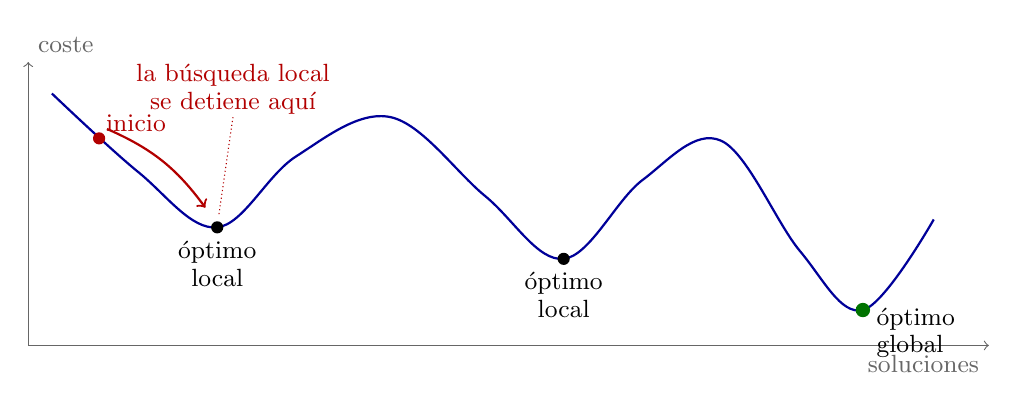
\begin{tikzpicture}[x=1cm,y=1cm]
  \draw[->,black!60] (0,0) -- (12.2,0) node[below left] {\small soluciones};
  \draw[->,black!60] (0,0) -- (0,3.6) node[above right] {\small coste};
  \draw[thick,blue!60!black] plot[smooth,tension=0.6] coordinates
     {(0.3,3.2) (1.4,2.2) (2.4,1.5) (3.4,2.4) (4.6,2.9) (5.8,1.9) (6.8,1.1) (7.8,2.1)
      (8.8,2.6) (9.8,1.2) (10.6,0.45) (11.5,1.6)};
  \fill[red!70!black] (0.9,2.63) circle (2.2pt) node[above right=-1pt] {\small inicio};
  \fill (2.4,1.5) circle (2.2pt);
  \node[below,align=center] at (2.4,1.45) {\small óptimo\\[-2pt]\small local};
  \fill (6.8,1.1) circle (2.2pt);
  \node[below,align=center] at (6.8,1.05) {\small óptimo\\[-2pt]\small local};
  \fill[green!45!black] (10.6,0.45) circle (2.6pt);
  \node[below right,align=left] at (10.65,0.6) {\small óptimo\\[-2pt]\small global};
  \draw[->,red!70!black,thick] (1.0,2.75) to[bend left=15] (2.25,1.75);
  \node[red!70!black,align=center] at (2.6,3.25) {\small la búsqueda local\\[-2pt]\small se detiene aquí};
  \draw[red!70!black,densely dotted] (2.6,2.9) -- (2.42,1.65);
\end{tikzpicture}
\caption{Una búsqueda local baja hasta el óptimo local más cercano y ahí se queda, aunque
haya soluciones mejores más lejos. Las metaheurísticas son distintas maneras de salir de ese
valle.}
\label{fig:paisaje}
\end{figure}

La figura~\ref{fig:paisaje} muestra la limitación fundamental de la búsqueda local: se
detiene en el primer óptimo local que encuentra. Las cinco metaheurísticas de la práctica son
cinco respuestas distintas a la pregunta \emph{¿cómo salgo de un óptimo local?}:

\begin{center}
\begin{tabular}{@{}lp{11cm}@{}}
\toprule
Metaheurística & Cómo escapa del óptimo local \\ \midrule
Temple Simulado & Acepta a veces movimientos que empeoran, con una probabilidad que va
                  disminuyendo. \\
Búsqueda Tabú & Hace siempre el mejor movimiento aunque empeore, y \emph{prohíbe} deshacer
                  los movimientos recientes para no volver atrás. \\
GRASP & No intenta escapar: vuelve a empezar desde otra solución inicial distinta, construida
                  con algo de azar. \\
Algoritmo Genético & Trabaja con muchas soluciones a la vez y las combina entre sí. \\
VNS & Cambia de estructura de entornos y da ``saltos'' cada vez mayores. \\
\bottomrule
\end{tabular}
\end{center}

\subsection{Intensificar y diversificar}

Todo buen heurístico tiene que equilibrar dos tendencias opuestas:
\begin{itemize}
  \item \textbf{Intensificar}: explotar a fondo la zona donde se han encontrado buenas
        soluciones (buscar cerca de lo mejor que se conoce).
  \item \textbf{Diversificar}: explorar zonas nuevas, alejadas de lo ya visitado.
\end{itemize}
Si solo se intensifica, el algoritmo se estanca enseguida; si solo se diversifica, es una
búsqueda al azar. Casi todos los parámetros que se calibran en la
sección~\ref{sec:calibracion} regulan precisamente este equilibrio (la temperatura del
temple, la duración tabú, el tamaño de la lista de candidatos de GRASP, la probabilidad de
mutación del genético o el tamaño del salto de la VNS).

\subsection{Clasificación}

Los apuntes clasifican las metaheurísticas en \textbf{trayectoriales} (manejan una única
solución que va cambiando: describe una trayectoria) y \textbf{poblacionales} (manejan un
conjunto de soluciones). De las cinco de la práctica, el Temple Simulado, la Búsqueda Tabú,
GRASP y la VNS son trayectoriales; el Algoritmo Genético es poblacional.

Como lectura complementaria general, gratuita y escrita para no especialistas, se recomienda
el libro de Luke~\cite{luke}, que figura en la bibliografía de los apuntes.
